% ---------------------------------------------------------------------
% 11_tres_patas.tex
% Diagrama de Venn "Las tres patas del análisis de datos" (bloque 1).
% Rehecho a partir de anterior/imagenes/3patas.png (@AnaBayes, sobre el
% diagrama de Drew Conway): los iconos de las intersecciones se
% sustituyen por sus etiquetas.
% Se compila aparte:   make img/tres_patas.pdf
% ---------------------------------------------------------------------
\documentclass[border=4pt]{standalone}
\usepackage[utf8]{inputenc}
\usepackage[T1]{fontenc}
\usepackage{mathpazo}
\usepackage{tikz}

\definecolor{comp}{HTML}{E57373}
\definecolor{area}{HTML}{9CCC65}
\definecolor{mate}{HTML}{64B5F6}
\definecolor{riesgo}{HTML}{8B0000}   % rojo oscuro: ¡cuidado!

\begin{document}
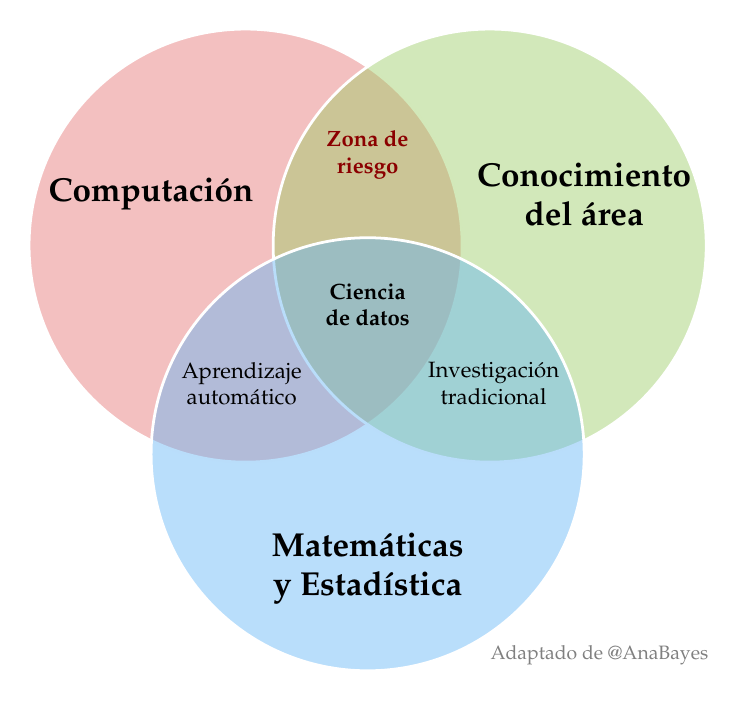
\begin{tikzpicture}[
    circulo/.style={fill opacity=0.45, draw=white, line width=1pt},
    pata/.style={font=\large\bfseries, align=center},
    cruce/.style={font=\footnotesize, align=center}]
  \def\r{2.75}
  \fill[comp, circulo] (-1.55, 0.90) circle (\r);
  \fill[area, circulo] ( 1.55, 0.90) circle (\r);
  \fill[mate, circulo] ( 0.00,-1.75) circle (\r);
  % las tres patas
  \node[pata] at (-2.75, 1.55) {Computación};
  \node[pata] at ( 2.75, 1.55) {Conocimiento\\del área};
  \node[pata] at ( 0.00,-3.20) {Matemáticas\\y Estadística};
  % intersecciones
  \node[cruce, font=\footnotesize\bfseries, text=riesgo] at ( 0.00, 2.05) {Zona de\\riesgo};
  \node[cruce] at (-1.60,-0.85) {Aprendizaje\\automático};
  \node[cruce] at ( 1.60,-0.85) {Investigación\\tradicional};
  \node[cruce, font=\footnotesize\bfseries] at (0.00, 0.15) {Ciencia\\de datos};
  % créditos
  \node[font=\scriptsize, text=gray, anchor=south east] at (4.45,-4.55)
    {Adaptado de @AnaBayes};
\end{tikzpicture}
\end{document}
